\documentclass[10pt]{article}
\usepackage[margin=0.75in]{geometry}
\usepackage{graphicx,booktabs,hyperref}
\hypersetup{colorlinks=true,urlcolor=blue}
\title{Point-driven pencil: one 28-bit target}
\author{Exploratory operation-count record}
\date{21 October 2026}
\begin{document}
\maketitle
\noindent\textbf{Scope.} Prime $p=48{,}383$, target index 0 from the frozen
28-bit source cohort. This is one cold-priced target, not a 60-target curve
or 1,260-target cohort result. Both the pencil scalar and same-process
source-negation-rho scalar passed source multiplication. A second archive-input
process matched every non-wall field and an independent native validator
recomputed both source scalars, the five summary prices and bounds, and all
36 pencil/rho pricing cells.

The pencil collector recorded 23,639 verified three-point relations,
20,814,919,424 modular row updates, rank 23,638 and 9,658,483 stored
nonzero coefficients. Its setup was charged in full to this target.
The first-run and replay L0 wall diagnostics were 1,723.90 and 1,668.79
seconds; neither is used in the prices.
\begin{center}\small
\begin{tabular}{lrr}
\toprule
Price: $M+0.5S+10I$, 0.1 GAE/native & Complete GAE & Pencil/rho \\
\midrule
Pencil & 6,245,360,741.03 & 96,957.132823 \\
Matched rho & 64,413.63 & 1.000000 \\
\bottomrule
\end{tabular}
\end{center}
Across the 36 pricing cells, 0/36 pencil ratios are below rho. The minimum
and maximum are 26.422722 and 113,636.290374, respectively. These are
single-target prices and do not estimate a 28-bit curve slice.
\begin{center}
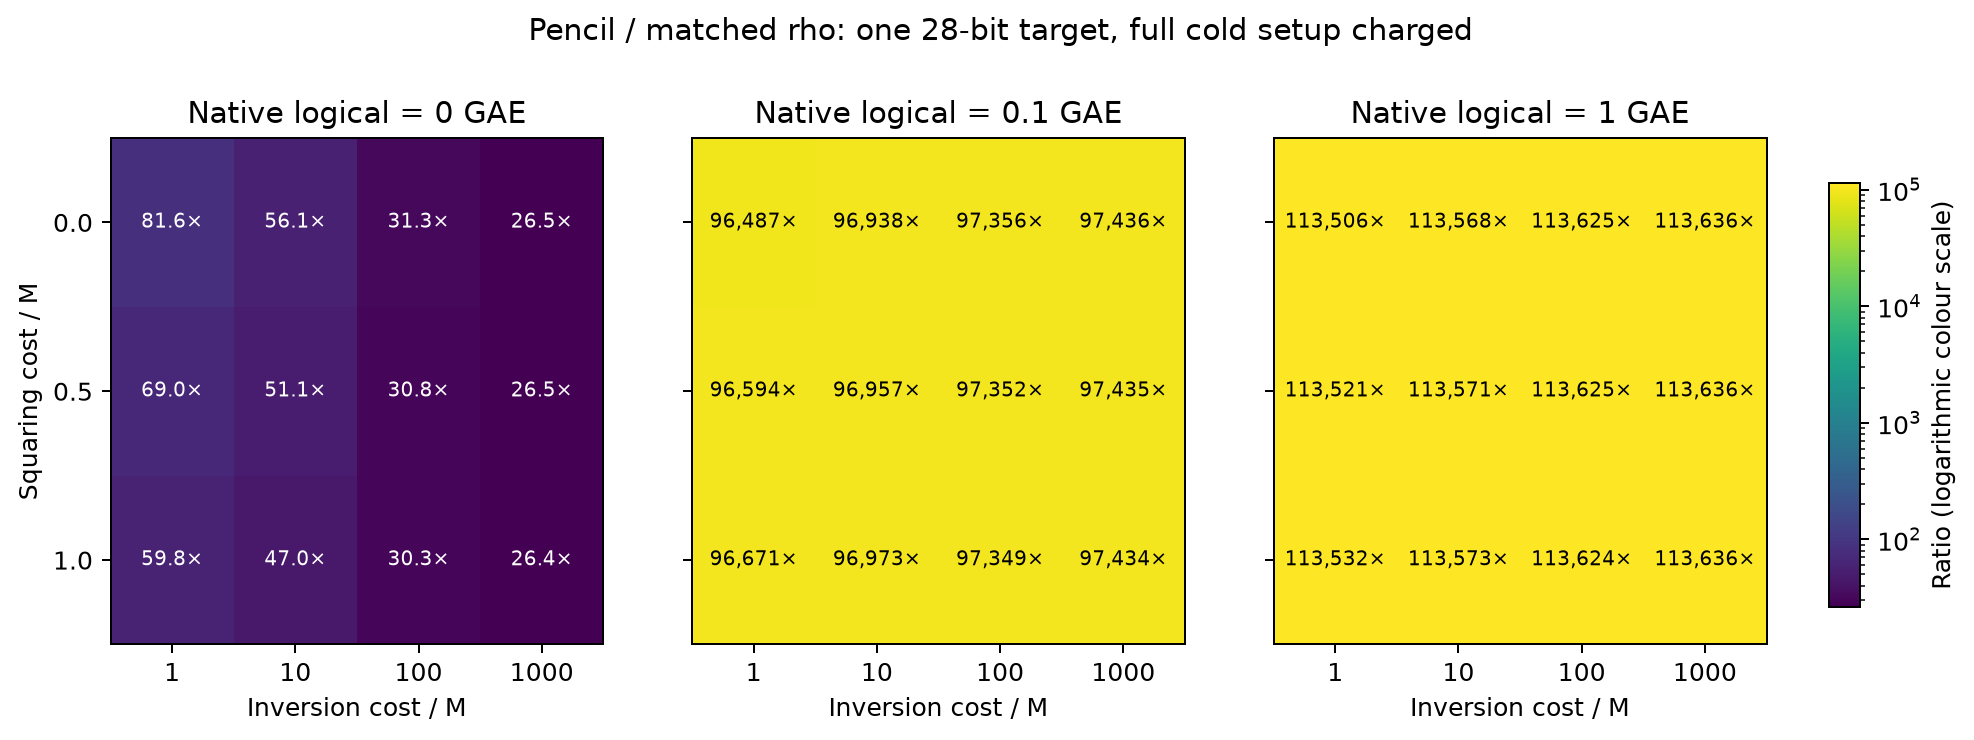
\includegraphics[width=0.98\linewidth]{pencil-one-target-grid.png}
\end{center}
\noindent Machine data: \path{results/pencil-pilot/}.
The files share the prefix \texttt{f48383}.

\noindent The nine complete smaller-curve pilots and their 540 independent
replays are in the \href{PENCIL_PILOT.pdf}{nine-curve report}.
\end{document}
